\documentclass[14pt,russian]{extreport}
\usepackage[utf8]{inputenc}
\usepackage{geometry}
%\geometry{verbose,tmargin=2cm,bmargin=2cm,lmargin=2cm,rmargin=2cm}
\geometry{verbose,tmargin=2.0cm,bmargin=2.0cm,lmargin=3.0cm,rmargin=2.0cm}
%\geometry{verbose,tmargin=3cm,bmargin=3cm,lmargin=3cm,rmargin=3cm}

\usepackage{amssymb}
\usepackage{setspace}
\usepackage{babel}
\usepackage{color}
\usepackage[hidelinks]{hyperref}
\usepackage{natbib}
%\usepackage{authordate1-4}
%\bibliographystyle{authordate1}
\bibliographystyle{unsrt}
\usepackage{amsmath}
\newtheorem{hyp}{Гипотеза}
\usepackage{graphicx}
\graphicspath{{img/}}
\usepackage{float}
\usepackage{placeins}
\usepackage{chngcntr}
\counterwithout{figure}{chapter}
\counterwithout{table}{chapter}
\usepackage{multicol}
\usepackage{tabularx,ragged2e,booktabs,caption}

\usepackage{pgfplots}
\usepackage{pgfplotstable}
\pgfplotsset{compat = 1.7}
\usepackage{filecontents}

\usepackage{booktabs}
%\usepgfplotslibrary{external} 
%\tikzexternalize
\pgfplotsset{compat=newest}

\usepackage{CJKutf8}
%\onehalfspacing
\linespread{1.5}

% remove chapter number from section headings
\renewcommand*\thesection{\arabic{section}}

\newcommand{\KG}{\textbf{KaGa}}
\newcommand{\BS}{\textbf{BigSmall}}
\newcommand{\MX}{\textbf{Mix}}

\usepackage{amsmath}
\DeclareMathOperator*{\argmin}{argmin}
\DeclareMathOperator*{\argmax}{argmax}
\newcommand*{\argminl}{\argmin\limits}
\newcommand*{\argmaxl}{\argmax\limits}

% rename chapters
\makeatletter
\renewcommand{\@chapapp}{Глава}
\makeatother

% continuous equation numbering through chapters
\usepackage{chngcntr}
\counterwithout{equation}{chapter}

\usepackage{cleveref}

\usepackage{caption}

\usepackage{amsthm}
\theoremstyle{definition}
\newtheorem{definition}{Определение}[subsection]

\usepackage{indentfirst}
\frenchspacing

\newcommand{\todo}[1]{}
\renewcommand{\todo}[1]{{\color{red} TODO: {#1}}}

\newcounter{appx}
\renewcommand{\theappx}{\Asbuk{appx}}

\newcommand{\intro}[1]{
	\stepcounter{section}
	\section*{Приложение \Asbuk{section}. #1}
	\addcontentsline{toc}{section}{Приложение \Asbuk{section}. #1}
	\refstepcounter{appx}
}

\begin{document}
	
\begin{titlepage}
	\begingroup
	\centering
	{\scshape
		\fontsize{12pt}{14pt}\selectfont Министерство образования и науки Российской Федерации\par
		\vspace{0.7cm}
		Государственное образовательное учреждение \\высшего профессионального образования\par
		Московский физико-технический институт\\(государственный университет)\par
		\vspace{0.7cm}
		Факультет инноваций и высоких технологий\par
		Кафедра компьютерной лингвистики\par
		\vspace{0.7cm}
		\fontsize{14pt}{17pt}\selectfont выпускная квалификационная работа\\(бакалаврская работа)\par}
	\fontsize{14pt}{17pt}\selectfont по направлению 01.03.02 «Прикладная математика и информатика»\par
	\vspace{1cm}
	{\fontsize{21pt}{25pt}\selectfont\bfseries Японский. Буквенные n-грамы \\ для распознавания\par}
	\vspace{4cm}
	
	\begin{tabular}{l@{\hspace{140pt}}r}
		Студент & Куликов А.В. \\
		Научный руководитель & Андрианов А.И.
	\end{tabular}
	\par
	\vfill
	
	{\fontsize{14pt}{17pt}\selectfont Москва, 2017\par}
	\endgroup
\end{titlepage}
\onehalfspacing

\addtocounter{page}{1}
\tableofcontents{}

\newpage
\section*{Введение}
\addcontentsline{toc}{section}{Введение}

История попыток распознать текст началась более века назад. В 1914 году Эмануэль Гольдберг разработал устройство, которой считывало символы и транслировало их в телеграфный код. Примерно в то же время ирландский химик Эдмунд Фурнье д’Альбе создал и запатентовал «оптофон» — прибор, умеющий переводить написанное в систему звуков, различающихся по высоте. Оптофон предназначался для того, чтобы слепые могли «читать».

В 1929 году Густав Таушек (Gustav Tauschek) разработал метод оптического распознавания текста. Машина Таушека представляла собой механическое устройство, которое использовало шрифтовые шаблоны и фотодетектор. Он запатентовал своё изобретение сначала в Германии, а позднее и в США, в 1935 году. Это и положило начало проблеме качественного оптического распознавания символов (Optical Character Recognition, OCR).

Коммерческое производство подобных маних было налажено уже в 1950-х, после войны. Использовавшие наработки военных, производители OCR-машин продвигались всё дальше, увеличивая применимость технологии и качество распознавания.

Постепенно появлялись как универсальные OCR-программы (ABBYY FineReader, Adobe Acrobat), так и специализированные для конкретной области (SmartScore для нотной записи, Persian Reader для фарси и т.д.). При этом точность в задаче распознавания напечатанных латинских символов достигла 99\%-100\% качества, в то время как корректное распознавание рукописного текста или текста, написанного в другом алфавите, до сих пор является темой множества исследований. Особняком стоит задача распознавания текста на восточных языках (CJK: китайский, японский, корейский), из-за большого размера алфавита в этих языках.

Настоящая работа представляет собой сравнение некоторых методов машинного обучения для исправления ошибок распознавания текста в японском языке. 

Спектр способов, которыми можно решать проблему автоматического исправления ошибок, довольно широк, и включает в себя различные вариации $n$-граммных моделей ($n$-gram models), использование нейросетей (Neural Networks, NN), скрытых моделей Маркова (Hidden Markov Models, HMM) и прочих методов машинного обучения. Более подробный обзор основных современных подходов можно найти в \cite{das:survey}.
 
Среди возможных решений использование $n$-граммных моделей занимает особую нишу из-за относительной прозрачности и интуитивности принципов работы, и в то же время достаточно широких возможностей по настройке алгоритма.

Подход, предложенный в \cite{nagata:shape}, использует $n$-граммные модели, а также различные алгоритмы сглаживания для исправления опечаток, опираясь на словное деление текста. 

В работе \cite{nagata:context} также даются эвристики для определения границ слов, использующие граф линейного деления (ГЛД). Эти границы слов затем используются в $n$-граммной модели в качестве вспомогательного контекста.

Более подробно эти и другие подходы разобраны в соответствующем разделе (\cref{sec:litreview}).

Данное исследование призвано рассмотреть некоторые из $n$-граммных моделей и сравнить их эффективность в задаче исправления опечаток в японском языке.

Актуальным приложением этой работы является система распознавания восточных языков в ABBYY FineReader.

\newpage

\section{ Постановка задачи }\label{sec:taskdef}

\begin{definition}{\textit{Оптическое распознавание символов (Optical Character Recognition, OCR)}} -- процесс считывания текста с физического носителя и его сохранения в цифровом формате. Текст состоит из \textit{символов}.
\end{definition}

\begin{definition}{\textit{Ошибка OCR}} -- случай, когда очередной символ текста распознался неверно или не распознался. Ведёт к понижению качества распознавания.
\end{definition}

\begin{definition}{\textit{$N$-грамма}} -- последовательность из $n$ элементов (слов, звуков, символов). Анализируя их частотности, можно строить модели для анализа и синтеза языка.
\end{definition}

\begin{definition}{\textit{$N$-граммная модель}} -- вероятностная модель языка, которая рассчитывает вероятность последнего элемента $n$-граммы, если известны все предыдущие. \\
При использовании $n$-граммных моделей предполагается, что появление каждого элемента зависит только от предыдущих элементов.
\end{definition}

\textbf{Цель работы} -- сравнить эффективность различных символьных $n$-граммных моделей в задаче исправления ошибок OCR в японском языке.

Из цели работы вытекают следующие \textbf{задачи}:
\begin{itemize}
	\item Рассмотреть существующие подходы к $n$-граммному моделированию японского языка;
	
	\item Реализовать некоторые символьные $n$-граммные модели;
	
	\item Развернуть систему для тестирования и сравнения моделей.
\end{itemize}

Чтобы понять специфику цели работы, нужно учесть особенности японского языка.

Очевидно, что устройство японского языка на уровне конкретных символов сложнее, чем устройство языков латино-романской группы, в которых существует всего 25-40 символов, учитывая возможную диакритику.

\subsection{ Обзор японского языка }
\label{sec:japanese}

Письменный японский текст -- это комбинация слогово-фонетических символов (кана) и иероглифов (кандзи).
Слоговая азбука кана делится на катакану и хирагану, которые представляют собой разные графические формы одних и тех же слогов.

Рассмотрим эти символы подробнее:

\begin{itemize}
	\item Хирагана (см. \cref{fig:hirag_sample}). В основном используется для образования грамматических морфем.
	\begin{figure}[H]
		\centering
		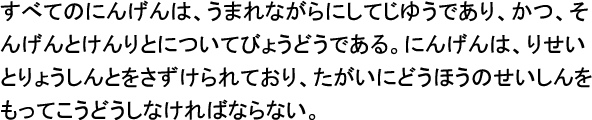
\includegraphics{hirag_sample.png}
		\caption{Хирагана}
		\label{fig:hirag_sample}
	\end{figure}
	
	\item Катакана (см. \cref{fig:katak_sample}). Используется для транскрибирования иностранных заимствованных слов.
	\begin{figure}[H]
		\centering
		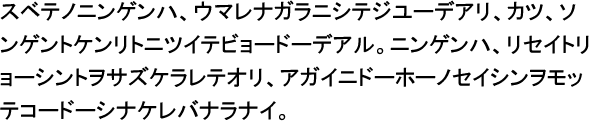
\includegraphics{katak_sample.png}
		\caption{Катакана}
		\label{fig:katak_sample}
	\end{figure}

\newpage
	\item Также есть диакритические символы -- дакутен, хандакутен (см. \cref{fig:dakut_sample_hir} и \cref{fig:dakut_sample_kat}). Они могут применяться как к катакане, так и к хирагане, и определённым образом влияют на звучание слогов.
	\begin{multicols}{2}
		
		\begin{figure}[H]
			\centering
			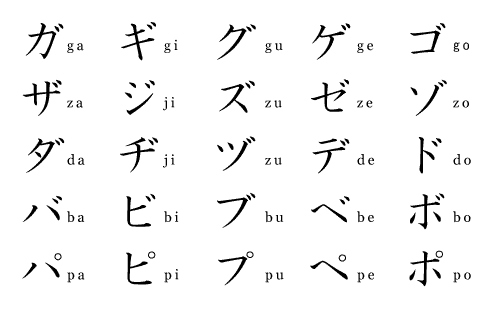
\includegraphics[scale=0.6]{dakut_sample.png}
			\caption{Дакутен катакана}
			\label{fig:dakut_sample_hir}
		\end{figure}
		
		\begin{figure}[H]
			\centering
			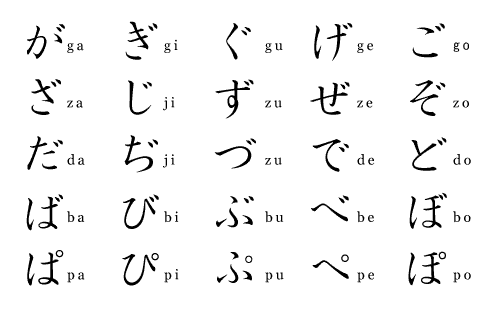
\includegraphics[scale=0.6]{handakut_sample.png}
			\caption{Дакутен хирагана}
			\label{fig:dakut_sample_kat}
		\end{figure}
		
	\end{multicols}
	
	\item Кандзи (см. \cref{fig:kandji_sample}). Это символы, несущие семантическую нагрузку.
	\begin{figure}[H]
		\centering
		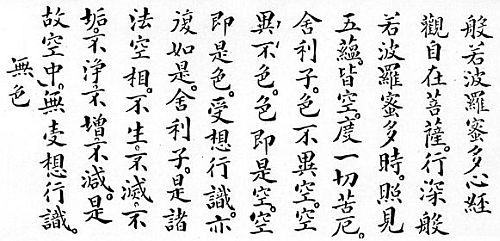
\includegraphics{kanji_sample.png}
		\caption{Кандзи}
		\label{fig:kandji_sample}
	\end{figure}
\end{itemize}

Кана различает 46 слогов, которые могут записываться как катаканой, так и хираганой. А вот иероглифов кандзи существует гораздо больше: 2136 (т.н. jōyō kanji -- "обычно используемые кандзи") достаточно для жизни, 6879 используется в кодировке JIS X 0208 (Japanese Industrial Standart, см. \cite{JISX0208}), а самые большие словари иероглифов (например, Большой китайско-японский словарь) включают в себя от 50000 до 85000.

Кроме перечисленных символов, в японском тексте могут быть и другие: фуригана -- маленькие знаки каны в качество фонетических подсказок, ромадзи -- система транслитерации японских слов в латиницу и т.д. Однако, в данной работе эти разделы оставлены за кадром.

Японский текст записывается с помощью комбинаций кандзи, кан и пунктуации, при этом отсутствует пробельное деление предложений на слова (см. \cref{fig:japtext_sample}).
	\begin{figure}[H]
	\centering
	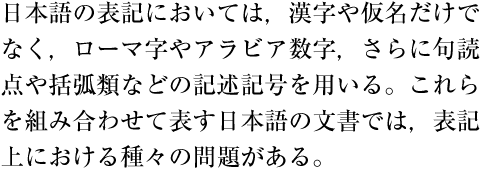
\includegraphics{japtext_sample.png}
	\caption{Японский текст}
	\label{fig:japtext_sample}
\end{figure}

По сравнению с латино-романскими языками, где алфавит меньше в сотни раз, а деление текста на слова очевидно, задача корректного распознавания символов становится значительно сложнее. Это требует более изощрённых подходов для автоматического анализа распознанного текста и поиска ошибок в нём.

Рассмотрим несколько примеров символов, которые легко спутать.

\subsection{ Путающиеся символы в японском }

При таком большом размере алфавита частые ошибки OCR можно разбить по классам. Вот некоторые из них:

\begin{itemize}
	\item[\textbf{2Kana}] 2 похожие каны. Таких случаев достаточно мало, а методы их различения уже существуют (см., например, метод с использованием глубокого обучения и свёрточных нейронных сетей в работе \cite{tsai:dcnn}).
	\begin{figure}[H]
		\center{\raisebox{-.5\height}{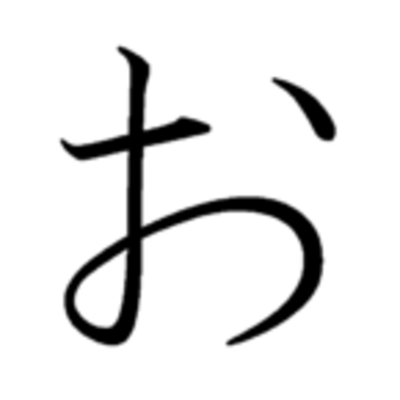
\includegraphics[height=100pt]{KanaO.png}}\ и \raisebox{-.5\height}{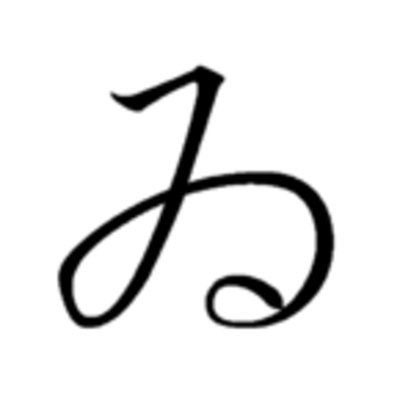
\includegraphics[height=100pt]{KanaWi.png}}}
	\end{figure}

	\item[\KG] Кана может легко путаться с соответствующим ей дакутен-символом.
	\begin{figure}[H]
		\center{\raisebox{-.5\height}{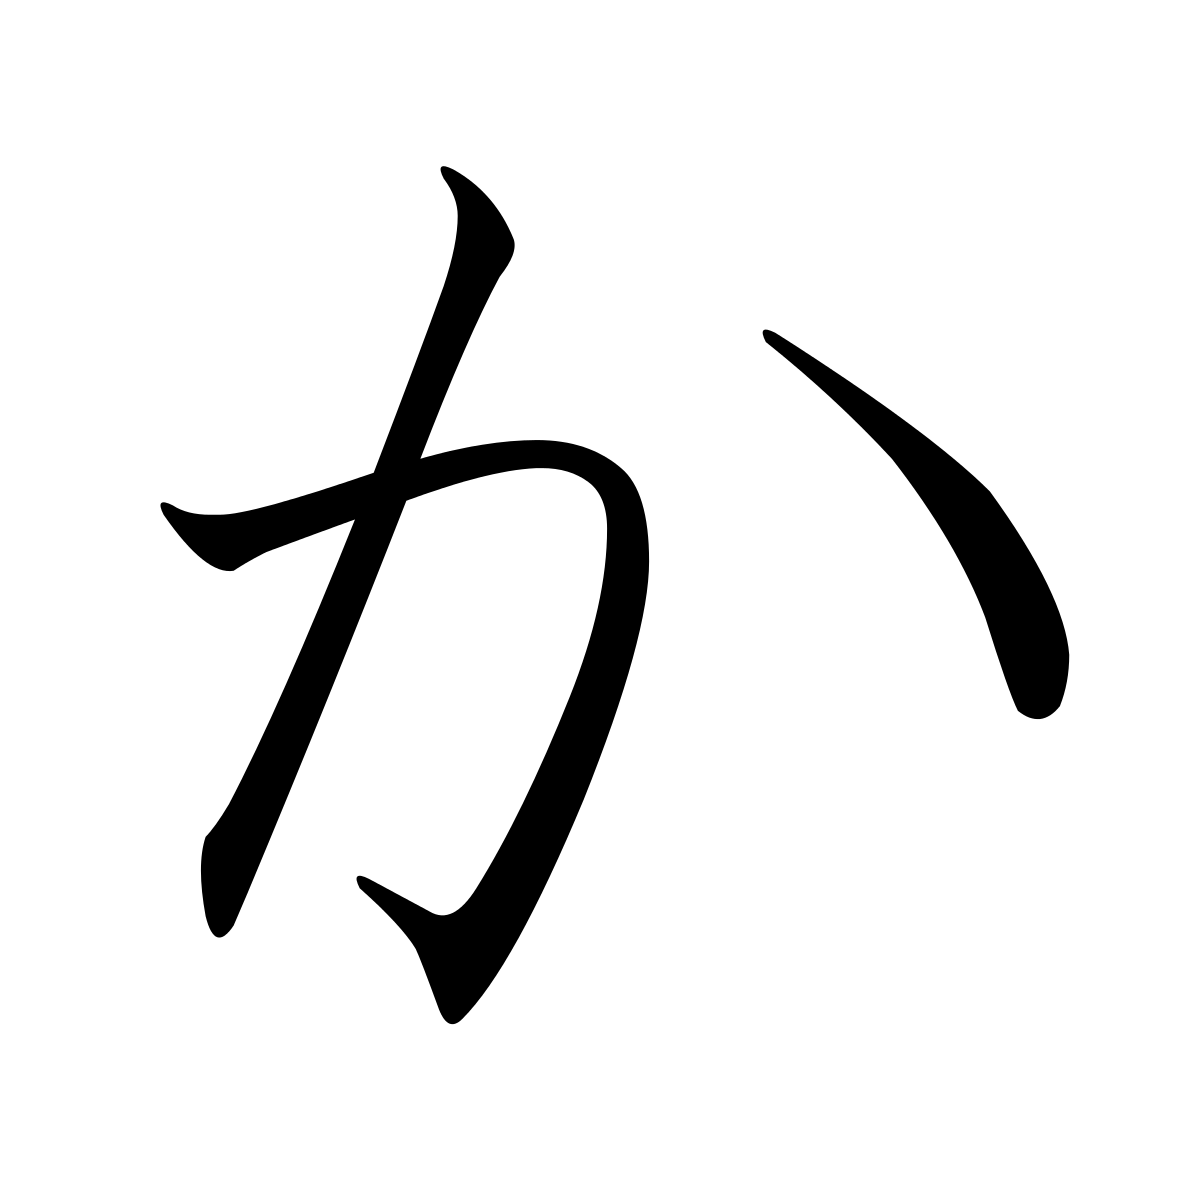
\includegraphics[height=100pt]{KanaKa.png}}\ и \raisebox{-.5\height}{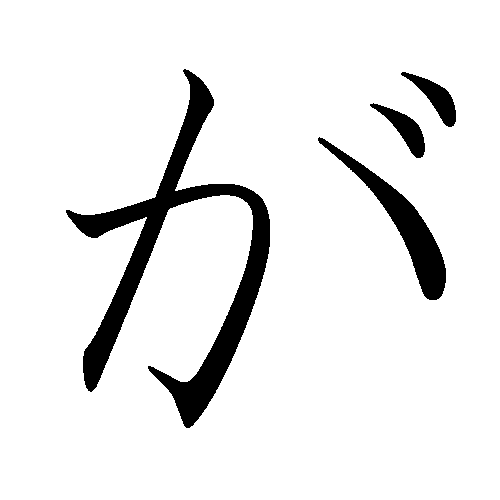
\includegraphics[height=100pt]{KanaGa.png}}}
	\end{figure}

	\item[\BS] Существуют большие и маленькие каны, которые нужно различать.
	\begin{figure}[H]
		\center{\raisebox{-.5\height}{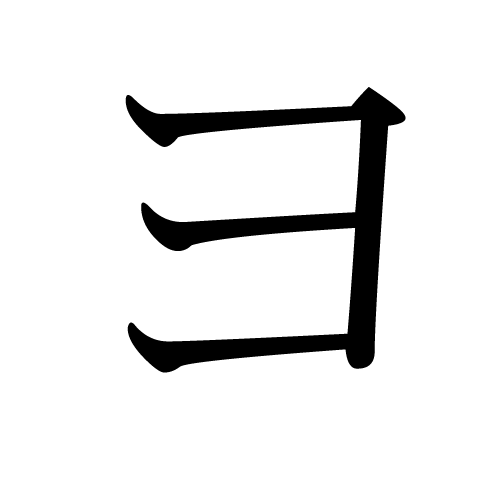
\includegraphics[height=100pt]{KanaYo.png}}\ и \raisebox{-.5\height}{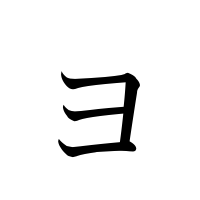
\includegraphics[height=100pt]{KanaYoSmall.png}}}
	\end{figure}
	
\end{itemize}

В будущем мы будем рассматривать 3 случая ошибок: \textbf{\KG}, \textbf{\BS} и \textbf{\MX} (смесь \textbf{\KG} и  \textbf{\BS} ), более строгое определение которых будет дано в \cref{sec:experiment}.

\subsection{ Формальная постановка задачи }

\begin{definition}
	{\textit{Алфавит $\Sigma = \{ a, b, c, .. \}$}} -- множество символов в данном языке.
\end{definition}

\begin{definition}
	{\textit{Текст $Text \in \Sigma^+$}} -- последовательность символов из алфавита $\Sigma$ положительной длины.
\end{definition}

\begin{definition}
	Текст делится на конечное число {\textit{предложений $S = \{ S_1, S_2, S_3, ... \}$}} знаками пунктуации и форматированием. $Text = S_1S_2S_3...$.
\end{definition}

Для каждого из предложения текста существует единственно верный вариант написания, а также некоторое (фиксированное) число неверных. Требуется ответить, какой из вариантов верен.

\begin{definition}
	{\textit{Оценивающий алгоритм (estimator) $\Theta : S \rightarrow \mathbb{R}^+ $}} -- функция, возвращающая оценку правильности варианта $S$.
\end{definition}

Среди $k$ вариантов предложения выбирается наилучший: $S_{best} = \argmaxl_{S} \Theta(S)$, который и считается правильным.

Если $S_{best}$ угадано верно, то на данном предложении алгоритм $\Theta$ отработал правильно.

\begin{definition}
	{\textit{Качество алгоритма $Q(\Theta) = \dfrac{\#\{ \text{угаданных предложений} \}}{\#\{ \text{всего предложений} \}}$}}.
\end{definition}

Задача -- реализовать ряд оценивающих алгоритмов (см. \cref{sec:models}), основанных на $n$-граммных моделях, и сравнить их по качеству.

\newpage
\section{ Обзор источников }\label{sec:litreview}

Проблема качественного OCR в различных языках (в частности, в японском) стоит достаточно давно, и существует множество различных подходов к её решению. Большинство подходов основываются на применении различных методов машинного обучения, такие как $n$-граммные модели, нейросети, модели Маркова и т.д. 

В силу особенностей японского языка (см. \cref{sec:japanese}), а именно отсутствия словного деления в текстах, существующие методы исправления ошибок OCR можно разделить на 2 класса: использующие информацию о словном делении и не использующие её.

\subsection{ Методы, не использующие словное деление }

Идея подобных методов заключается в том, чтобы, не тратя ресурсы на определение границ слов в тексте, оперировать предложениями (границы которых выделяются достаточно легко) как единицами трансляции, и исправлять возможные ошибки OCR, не углубляясь в членение предложений.

\todo{примеры статей?}

Стоит также заметить, что настоящая работа может быть отнесена к этому классу.

\subsection{ Методы, использующие словное деление }

Информация о словном делении текста даёт удобный контекст для выделения признаков и настройки параметров при машинном обучении. Но эту информацию надо откуда-то получать, что приводит к делению алгоритмов на 2 этапа:

\begin{itemize}
	\item Получение словного деления. Может производиться с помощью специализированных алгоритмов (например, модификаций алгоритма Витерби, как в \cite{nagata:context}, или марковских случайных полей (conditional random fields, CRFs), как в \cite{kudo:crfs}), а также путём анализа конкретных языковых конструкций (например, bunsetsu boundaries, см. \cite{chung:bunsetsu}).
	
	Кроме того, словное деление может быть получено путём использования в работе предварительно размеченного корпуса, в разметке которого есть словное деление. В качестве примеров таких корпусов можно привести EDR Japanese Corpus (см. \cite{corpus:edr}), ATR Dialogue Database (см. \cite{corpus:atr}) и т.д.
	
	\item Применение словного деления как контекста для детектирования ошибок OCR. Достоверная информация о словном делении позволяет считать слова единицами трансляции, не теряя контекста предложения. Это даёт возможность получить больше признаков для машинного обучения. Подобный подход представлен в статье \cite{nagata:shape}, где используются $n$-граммные модели с backoff и различными подходами к сглаживанию (Good-Turing, Witten-Bell). 
\end{itemize}

Обзору основных актуальных методов исправления ошибок OCR в японском также целиком посвящена статья \cite{das:survey}.

\newpage
\section{ Описание моделей оценивания текста }\label{sec:models}

Перед обучением моделей корпус разбивается на независимые и гомогенные части: обучающую и тестовую выборки. Обучающая выборка используется для обучения модели, тестовая -- для проверки качества обучения и, собственно, оценки модели.

В работе рассматриваются следующие модели: 

\begin{itemize}
	\item $n$-граммные с фиксированным $n,\ n \in \{1,2,3\}$
	
	\item Backoff-модель, $n_{max} \in \{ 3, 5, 7 \}$
	
	\item Модель Катца (Katz),  $n_{max} \in \{ 3, 5, 7 \}$
\end{itemize}

Также из-за большого размера алфавита необходимо использовать сглаживание (smoothing) для учёта символов и $n$-грамм, не встретившихся в обучающей выборке. Подробнее о механизме сглаживания -- см. раздел \cref{sec:experiment}.

Во всех моделях оценка предложения производится через агрегацию оценок отдельных $n$-грамм.

\subsection{ $N$-граммные модели с фиксированным $n$ }

\paragraph{ Обучение модели } Для данного $n$ по обучающей выборке собираются статистики по всем $n$-граммам. Эти статистики затем нормализуются и сериализуются для дальнейшего использования.

$$ C(x_{i - n + 1}, ..., x_{i - 1}, x_i) = \dfrac{N(x_{i - n + 1}, ..., x_{i - 1}, x_i)}{N(x_{i - n + 1}, ..., x_{i - 1})} $$ 

\paragraph{ Применение модели } В силу простоты модели оценка $n$-граммы из тестовой выборки берётся напрямую из собранных на предыдущем этапе статистик.

$$ P(x_i | x_{i - n + 1}, ..., x_{i - 1}) = C(x_{i - n + 1}, ..., x_{i - 1}, x_i) $$

\subsection{ Backoff-модель } 

\paragraph{ Обучение модели } Этап обучения модели практически такой же, как и в случае простой $n$-граммной модели, с разницей в том, что здесь собираются статистики для всех $n \leq n_{max}$.

\paragraph{ Применение модели } Идея backoff-подхода состоит в том, что при нехватке данных для оценки какой-либо $n$-граммы $x_{i - (n - 1)} ... x_{i - 1} x_i$ постепенно уменьшается $n$, что позволяет увеличить общность алгоритма и оценить $n$-грамму по частям, но более надёжно. За счёт этого уменьшается вероятность переобучения модели на конкретных данных. Подробнее можно узнать в \cite{manning}.

\[ P_n(x_i | x_{i - n + 1}, ..., x_{i - 1}) =
\begin{cases}
	C(x_i | x_{i - n + 1}, ..., x_{i - 1})       & \quad \text{if } C(x_i | x_{i - n + 1}, ..., x_{i - 1}) > k\\
	P_{n - 1}(x_i | x_{i - n + 2}, ..., x_{i - 1})  & \quad \text{otherwise }\\
\end{cases}
\]

\subsection{ Модель Катца (Katz) }

\paragraph{ Обучение модели } Этап обучения модели такой же, как и в случае backoff-модели.

\paragraph{ Применение модели } Модель Катца является улучшенной версией backoff-модели, в которой накладывается динамический дисконт (коэффициенты $d_{w_{i-n+1}...w_i}$ и $\alpha_{w_{i-n+1}...w_{i-1}}$) на оценку $n$-граммы в случае уменьшения $n$. Более подробно о модели Катца можно прочитать в \cite{katz:backoff}.

\[
P_{n}\left( w_i | w_{i-n+1}...w_{i-1} \right) = 
\begin{cases}
d_{w_{i-n+1}...w_i} \dfrac{C(w_{i-n+1}...w_i)}{C(w_{i-n+1}...w_{i-1})} &\text{if $C(w_{i-n+1}...w_i) > k$}\\
\alpha_{w_{i-n+1}...w_{i-1}} P_{n - 1}\left( w_i | w_{i-n+2}...w_{i-1} \right) &\text{otherwise}
\end{cases}
\]

При этом коэффициенты $d_{w_{i-n+1}...w_i}$ и $\alpha_{w_{i-n+1}...w_{i-1}}$ вычисляются следующим образом:

$$d_{w_{i-n+1}...w_i} - \text{ размер дисконта, вызванного сглаживанием (см. \cref{sec:experiment}) }$$

$$\alpha_{w_{i-n+1}...w_{i-1}} - \text{ размер дисконта за backoff } -$$ 
$$ = \dfrac{\beta_{w_{i-n+1}...w_{i-1}}}{\Sigma_{\{ w_i : C(w_{i-n+1}...w_{i-1}) \leq k \}} P_{n-1}\left( w_i | w_{i-n+2}...w_{i-1} \right)}\text{,}$$

$$\text{где } \beta_{w_{i-n+1}...w_{i-1}} - \text{ остаточная плотность вероятности для ($n-1$)-грамм } - $$
$$ = 1 - \Sigma_{\{ w_i : C(w_{i-n+1}...w_{i}) > k \}} \dfrac{C(w_{i-n+1}...w_i)}{C(w_{i-n+1}...w_{i-1})} $$ \todo{проверить N или C тут}


\newpage
\section{ Описание эксперимента }\label{sec:experiment}

Для исследования способов исправлять ошибки OCR в тексте необходимо либо иметь большой корпус размеченных данных с результатами распознавания, либо как-то выкручиваться. 

Пришлось выкручиваться, эмулируя ошибки OCR самостоятельно.

\todo{Описание машины -- в приложение}

\subsection{ Корпус }

Для обучения и сравнения $n$-граммных моделей использовался корпус html-страниц с ряда японских сайтов (\todo{Каких? Где?}) общим размером $\approx 8,5 GB$. 

Тексты из этого корпуса не были результатом OCR, поэтому в них не должно было быть ошибок, связанных с распознаванием. Эти тексты были признаны верными с точки зрения языка и подходящими для обучения моделей.

В рамках подготовки корпуса к эксперименту тексты были перемешаны, чтобы тематика текста не зависела от его исходного положения в корпусе, из текстов были удалены html-теги, сложное форматирование, небольшое число мусорных символов. Также корпус был единообразно переведён в кодировку Unicode. Подробнее об этих технических этапах -- см. раздел \ref{sec:coding}.

После вышеперечисленных операций корпус был готов к использованию, его размер составлял $\approx 1,5 GB$. При этом размер алфавита в нашем корпусе составлял $\approx 7000$ символов, что в 3 раза меньше размера таблиц Unicode.

Имея данные, готовые к использованию, было бы глупо не построить по ним несколько графиков.

\subsection{ \todo{Zipf} }

Если посмотреть на распределение частот отдельных символов, то оно выглядело так:

\begin{figure}[H]
	\centering
	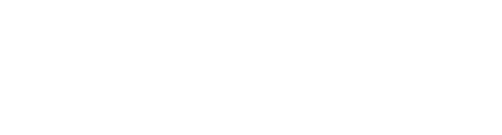
\includegraphics{draft.png}
	\caption{1gramstats}
	\label{fig:1gramstats_all}
\end{figure}

Видно, что распределение похоже на обратно экспоненциальное (кстати, это же утверждает закон Ципфа \todo{link}). Проверим эту гипотезу, построив график обратного логарифма (\todo{формулы}):

\begin{figure}[H]
	\centering
	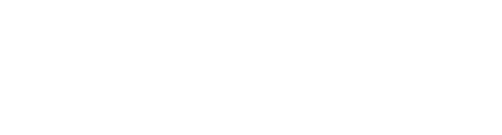
\includegraphics{draft.png}
	\caption{zipf}
	\label{fig:zipf1gram}
\end{figure}

Действительно, этот график с достаточной точностью ложится на прямую (\todo{погрешности?}). Тем самым, в NLP закон Ципфа проверен ещё раз.

Посмотрев на Рис. \ref{fig:1gramstats_all}, можно также заметить, что только очень малая часть символов появляется большое число раз. Посмотрим поближе на "голову"\ того же распределения:

\begin{figure}[H]
	\centering
	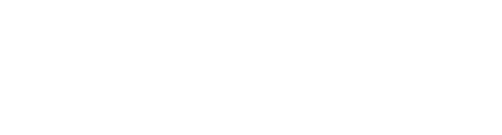
\includegraphics{draft.png}
	\caption{1gramstats head}
	\label{fig:gramstats_head}
\end{figure}

Действительно, лишь $\approx 200$ символов встречаются достаточно часто.

Осталюся ещё примерно $6500$ символов, которые входят в алфавит, но статистически мало отличаются от тех символов, что вовсе не встретились в нашем корпусе. Для оптимизации времени работы и занимаемой памяти эти символы можно представить более сжато.

\begin{definition}
	{\textit{Корзина (бакет, bucket)}} -- множество символов, которые считаются статистически малозначимыми и заменяются на U+FFFD (Unicode Replacement Character).
\end{definition}

Бакет $B_i$ характеризуется числом $|\Sigma_{B_i}|$ -- размером алфавита, который остаётся после сливания некоторого хвоста распределения в бакет. Было решено рассматривать бакеты с алфавитами размером $|\Sigma_{B_i}| = \{ 7000, 4800, 2600, 200 \}$, поскольку примерно на эти размеры алфавитов приходятся изменения в характере убывания частот символов.

На Рис. \ref{fig:bucket_pic} схематично изображено распределение частот после применения бакета с $|\Sigma_{B_i}| = 200$.

\begin{figure}[H]
	\centering
	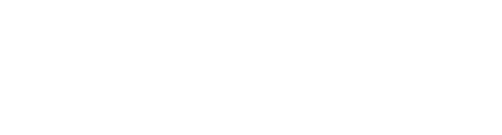
\includegraphics{draft.png}
	\caption{bucket}
	\label{fig:bucket_pic}
\end{figure}

Поскольку нам были недоступны корпуса текстов, распознанные какой-либо OCR машиной, было принято решение эмулировать ошибки OCR самим. Это делалось при помощи генератора шума.

\subsection{ Генератор шума и режимы его работы }

\begin{definition}
	{\textit{Шум $Noise = \{ (a_1, a_2), (b_1, b_2, b_3), (c_1, c_2), ... \}$}} -- множество наборов символов алфавита $\Sigma$, которые легко спутать при распознавании. Конкретные шумы определяются эмпирически. 
\end{definition}

Для эмуляции ошибок OCR был разработан скрипт -- генератор шума. Он параметризуется конкретным шумом и частотой его применения.

\begin{definition}
	{\textit{Генератор шума}} -- настраиваемый скрипт, который принимает эталонное предложение $S$, находит в нём символы-представители наборов конкретного шума $x \in S\ |\ \exists \xi = \{ \xi_1, \xi_2, ..., \xi_l \} \in Noise : x \in \xi$, и случайным образом меняет эти символы $x$ на "шумовые" из соответствующего набора $\xi$.
\end{definition}

С помощью шума $Noise$ случайным образом генерируются ошибки в предложениях текста $Text$. Таким образом происходит стохастическая эмуляция ошибок OCR. 

Тестовая часть корпуса была разбита на предложения (см. формальную постановку задачи в разделе \ref{sec:taskdef}), которые независимо друг от друга зашумлялись. Эти предложения после зашумления подавались на вход оценивающему алгоритму $\Theta$, который выбирал лучший из предложенных вариантов.

Были определены следующие шумы, обоснование выбора см. в разделе \ref{sec:taskdef}: 

\begin{itemize}
	\item[KaGa] Наборы симвопов, соответствующие добавлению диакритики. Например,
	
	\begin{multicols}{3}
		\begin{CJK}{UTF8}{min}
			かが \\
			きぎ \\
			くぐ \\
			けげ \\
			こご \\
			さざ \\
			しじ \\
			すず \\
			ふぶぷ   \\
			そぞ \\
			ただ \\
			なに \\
			たな \\
			だな \\
			んだ \\
			ちぢ \\
			つづ \\
		ほぼぽ \end{CJK}
	\end{multicols}
	
	\item[HalfWidth] Полуширинные/полноширинная катакана:
	
		\begin{multicols}{3}
		\begin{CJK}{UTF8}{min}
				ヲヲ\\
			ァァ\\
			ィィ\\
			ゥゥ\\
			ェェ\\
			ォォ\\
			ャャ\\
			ュュ\\
			ョョ\\
			ッッ\\
			ーー\\
			アア\\
			イイ\\
			ウウ\\
			エエ\\
			オオ\\
			カカ\\
			キキ  \end{CJK}
	\end{multicols}
	


	\item[BigSmall] Большие/маленькие написания букв:
	
	\begin{multicols}{3}
	\begin{CJK}{UTF8}{min}
		あぁ \\
		いぃ\\
		うぅ\\
		えぇ\\
		おぉ\\
		つっ\\
		やゃ\\
		ゆゅ\\
		よょ\\
		わゎ\\
		アァ\\
		イィ\\
		ウゥ\\
		エェ\\
		オォ \end{CJK}
\end{multicols}

	\item[Mix] Комбинация предыдущих режимов.
		\begin{multicols}{3}
		\begin{CJK}{UTF8}{min}
			かが \\
			きぎ \\
			くぐ \\
			けげ \\
			こご \\
			ャャ\\
			ュュ\\
			ョョ\\
			ッッ\\
			ーー\\
			アア\\
			アァ\\
			イィ\\
			ウゥ\\
			エェ\\
			オォ \end{CJK}
	\end{multicols}
	
\end{itemize}

\todo{ Срез шума в Ципфе -- график }

Интересно понимать, как выглядит результат работы генератора шума.
Предположим, на вход генератору было дано следующее предложение:

\begin{CJK}{UTF8}{min}キャンペーンは終了致しました。 \end{CJK} 

Тогда для различных шумов и режима "1 символ на предложение" получались такие результаты, которые затем фиксировались.

\begin{tabular}{c|c}
	Шум 	& Текст (пер. с яп. Campaign has ended)\\
	Эталон 	& \begin{CJK}{UTF8}{min}キャンペーンは終了致しました。 \end{CJK} \\
	KaGa	&  \begin{CJK}{UTF8}{min}ギャンペーン\colorbox{yellow}{\textbf{ぱ}}終了致しました。 \end{CJK} \\
	HalfWidth &  \begin{CJK}{UTF8}{min}キャンペ\colorbox{yellow}{\textbf{ー}}ンは終了致しました。 \end{CJK} \\
	BigSmall &  \begin{CJK}{UTF8}{min}キ\colorbox{yellow}{\textbf{ヤ}}ンペーンは終了致しました。 \end{CJK} \\
	Mix 	&  \begin{CJK}{UTF8}{min}\colorbox{yellow}{\textbf{ギ}}ャンペーンは終了致しました。 \end{CJK} 
\end{tabular}

\subsection{ Baseline эксперимента }

В качестве бейзлайна эксперимента была выбрана униграммная модель ($n = 1$).

Для разных шумов она показала следующие результаты, $|\Sigma_{B_i}| = 4800$:

\begin{tabular}{c|c}
	Шум 	& Оценка модели \\ \hline
	KaGa	& 0.70  \\
	HalfWidth &  0.71 \\
	BigSmall & 0.77  \\
	Mix 	&  
\end{tabular}

\todo{достать и добавить результаты для остальных бакетов}


\newpage

\section{ Реализация модели }\label{sec:coding}

Из-за обилия задач, связанных с обработкой текста в Unicode, а также по причине наличия удобных специализированных библиотек в качестве основного языка программирования был выбран Python 3. Впрочем, отдельные задачи, связанные с предобработкой корпуса, писались на Bash. Для подробных спецификаций использованного софта см. \todo{приложение}.

\subsection{ Общее окружение: nltk, pygtrie }

Глобально эксперимент состоял из следующих этапов:

\begin{enumerate}
	\item Обучение модели:
	
	\begin{enumerate}
		\item Получение $n$-грамм для обучающей выборки;
		
		\item Подсчёт статистики по $n$-граммам;
		
		\item Сериализация статистики на диск;
	\end{enumerate}
	
	\item Применение модели:
	\begin{enumerate}
		\item Десериализация обученной модели;
	
		\item Получение $n$-грамм для тестовой выборки;
	
		\item Оценивание моделью различных вариантов написания для предложения;
		
		\item Вычисление оценки модели.
	\end{enumerate}	
\end{enumerate}

Поскольку в ходе эксперимента считались статистики по 7-граммам для корпуса из \todo{статистики по строкам?}, было необходимо хранить статистики эффективно. Для хранения строк подобного вида лучше всего подходит такая структура данных, как префиксное дерево (бор, trie).

Поскольку задачи писать эффективное и масштабируемое префиксное дерево не было, была выбрана его реализация, предоставленная Google в библиотеке pygtrie (см. \cite{python:pygtrie}, \cite{python:pygtrierepo}). \todo{нормально ли репозиторий в cite?}

Для получения $n$-грамм, а также различных вспомогательных задач был выбран популярный python-пакет nltk (Natural Language ToolKit, см. \cite{python:nltk})

\subsection{ Полезные утилиты }

\paragraph{ Pickle } Удобный модуль для сериализации/десериализации сложных Python-объектов.

\paragraph{ BeautifulSoup.UnicodeDammit } Спасительный модуль для работы с разнообразными кодировками в составе пакета BeautifulSoup. Особенно мощно работает в связке с библиотеками chardet и cchardet. Без него привести корпус к читабельному виду было бы невозможно.

В качестве подтверждения -- статистика по различным кодировкам в исходном корпусе:

\begin{tabular}{c|c}
Кодировка & Количество файлов \\ \hline 
utf-8 & 68789\\ 
iso-8859-2 & 46870\\ 
shift\_jis & 42015\\ 
euc-jp & 2562\\ 
cp932 & 1575\\ 
ascii & 544\\ 
windows-1253 & 436\\ 
iso-8859-7 & 256\\ 
windows-1252 & 78\\ 
iso-8859-5 & 9\\ 
gb2312 & 4\\ 
tis-620 & 4\\ 
ibm866 & 1\\ 
maccyrillic & 1\\ \hline
Всего & 163144
\end{tabular}

Документацию можно найти в \cite{python:dammit}.

\paragraph{ Graphviz } Простая утилита и язык для визуализации графов, полезно для вглядывания в префиксные деревья.

\subsection{ Пример работы и статистики }

\todo{ Разобрать предложение и пройтись по этапам визуализации результата (до svg-картинки с траем) -- если будет нужна красивая вода. }

\newpage
\section{ Результаты эксперимента }\label{sec:results}



\newpage

\section{ Анализ результатов }\label{sec:analysis}

\newpage
\section{ Заключение }\label{sec:epilogue}

В работе проанализированы некоторые модели машинного обучения, основанные на символьных $n$-граммах, эти модели были сравнены в качестве решений для автоматического исправления ошибок OCR. Исследования были проведены для различных характеров ошибок OCR, которые имитировались в процессе эксперимента.

Также были проведены измерения производительности этих подходов с точек зрения времени и памяти. В силу особенностей японского языка затраты памяти на работу с обученной 7-граммной моделью впечатляют.

Однако, менее глубокие модели требуют разумных объёмов ресурсов, показывая при этом хорошие результаты, сравнимые с показателями аналогичных работ, в которых результаты были получены с привлечением информации о словном делении, а также POS-тегов.

Возможными направлениями дальнейшего развития данной темы могли бы стать исследования с реальными ошибками OCR, оптимизация структур данных с целью использовать более полные статистики (например, 7-граммное префиксное дерево), реализация других моделей и алгоритмов (например, сглаживание по Кнезеру-Нею (Kneser-Ney)).

\newpage

\addcontentsline{toc}{section}{Список литературы}
\begin{thebibliography}{00}
	
\bibitem{das:survey} 
\textit{Soumendu Das et al.} Survey of Pattern Recognition Approaches in Japanese Character Recognition //\\
(IJCSIT) International Journal of Computer Science and Information Technologies, Vol. 5(1), 2014. P.~93~-~99.

\bibitem{nagata:shape} 
\textit{Nagata, Masaaki} Japanese OCR Error Correction using Character Shape Similarity and Statistical Language Model //\\
Proceedings of the 17th International Conference on Computational Linguistics - Volume 2, 1998. P.~922~-~928.

\bibitem{nagata:context} 
\textit{Nagata, Masaaki} Context-based Spelling Correction for Japanese OCR //\\
Proceedings of the 16th Conference on Computational Linguistics - Volume 2, 1996. P.~806~-~811.

\bibitem{katz:backoff} 
\textit{S. Katz} Estimation of probabilities from sparse data for the language model component of a speech recognizer. //\\
IEEE Transactions on Acoustics, Speech, and Signal Processing, vol. 35, no. 3, 1987. P.~400~-~401.

\bibitem{python:pygtrie} Pygtrie documentation [Электронный ресурс]. \\ URL: http://pygtrie.readthedocs.io/en/latest/ -- 2014

\bibitem{python:pygtrierepo} Pygtrie github [Электронный ресурс]. \\ URL: https://github.com/google/pygtrie -- 2017

\bibitem{python:nltk} Natural Language Toolkit [Электронный ресурс]. \\ URL: http://www.nltk.org/ -- 2017

\bibitem{python:dammit} Beautiful Soup Documentation [Электронный ресурс]. \\ URL: https://www.crummy.com/software/BeautifulSoup/bs4/doc/ -- 2015

\end{thebibliography}

\newpage

\appendix
\addtocontents{toc}{\protect\setcounter{tocdepth}{1}}
\renewcommand{\thesection}{\Asbuk{section}}

\intro{Условия эксперимента}

\singlespace

\subsection{ Аппаратные характеристики платформы }

\label{appendix:specs}

\begin{table}[H]
	\begin{center}
\begin{tabular}{|c|c|}\hline
	Архитектура            & x86-64   \\ \hline
	Частота процессора     & 3.30 GHz \\ \hline
	Количество процессоров & 32       \\ \hline
	Оперативная память     & 192 GB \\  \hline
\end {tabular}
\end{center}
\end{table}

\subsection{ Используемое программное обеспечение }
\begin{table}[H]
	\begin{center}
\begin{tabular}{|c|c|} \hline
	Python            &  3.5.2 64-bit  \\ \hline
	nltk &  3.2.4 \\\hline
	pygtrie & 2.1 \\\hline
	BeautifulSoup & 4.4 \\ \hline
\end {tabular}\end{center}
\end{table}

\renewcommand{\thesection}{\Asbuk{section}}

\intro{Результаты модели Катца для символов}
\subsection{ Результаты модели Катца для символов }

\label{appendix:table}
\begin{table}[H]
	\begin{center}
		\begin{CJK}{UTF8}{min}
		\begin{tabular}{ | l | l | l | l | l | l | l | l | l | }
			\hline
			Symbol & TP & FN & FP & TN & Precision & Recall & F1 & Accuracy \\ \hline
			な & 20554 & 185 & 802 & 127893 & 0.96244615096459996 & 0.99107960846713905 & 0.97655303480223299 & 0.99339507742548505 \\ \hline
			だ & 789 & 25 & 50 & 9853 & 0.94040524433849804 & 0.96928746928746901 & 0.95462794918330296 & 0.99300177288420199 \\ \hline
			ビ & 1300 & 80 & 10 & 306 & 0.99236641221374 & 0.94202898550724601 & 0.96654275092936803 & 0.94693396226415005 \\ \hline
			ピ & 403 & 6 & 67 & 712 & 0.85744680851063804 & 0.98533007334963296 & 0.91695108077360599 & 0.93855218855218803 \\ \hline
			ミ & 481 & 12 & 19 & 1229 & 0.96199999999999997 & 0.97565922920892401 & 0.96878147029204398 & 0.98219414129810401 \\ \hline
			マ & 1229 & 19 & 12 & 481 & 0.99033037872683305 & 0.98477564102564097 & 0.98754519887504999 & 0.98219414129810401 \\ \hline
			び & 43633 & 9 & 59 & 117 & 0.99864963837773502 & 0.99979377663718405 & 0.99922137998946503 & 0.99844812634077296 \\ \hline
			ひ & 229 & 63 & 5 & 21435 & 0.97863247863247804 & 0.784246575342465 & 0.87072243346007605 & 0.99687097367936595 \\ \hline
			の & 497614 & 9348 & 10 & 6194 & 0.99997990450621299 & 0.98156074814285799 & 0.99068471987465401 & 0.98176418546824995 \\ \hline
			め & 6194 & 10 & 9348 & 497614 & 0.398533007334963 & 0.99838813668600901 & 0.56966798491676596 & 0.98176418546824995 \\ \hline
			さ & 10916 & 24 & 0 & 228 & 1 & 0.99780621572212003 & 0.99890190336749596 & 0.99785100286532902 \\ \hline
			ざ & 228 & 0 & 24 & 10916 & 0.90476190476190399 & 1 & 0.95 & 0.99785100286532902 \\ \hline
			で & 42499 & 944 & 4 & 6954 & 0.99990588899607002 & 0.97827037727596999 & 0.98896981825797503 & 0.98119084938790901 \\ \hline
			て & 6954 & 4 & 944 & 42499 & 0.88047606989111105 & 0.99942512216154 & 0.93618739903069403 & 0.98119084938790901 \\ \hline
			に & 249152 & 1310 & 94 & 6978 & 0.999622862553461 & 0.99476966565786396 & 0.99719035916975496 & 0.99454829265262001 \\ \hline
			ぬ & 52 & 0 & 541 & 123404 & 8.7689713322090995E-2 & 1 & 0.16124031007751899 & 0.99563699121752902 \\ \hline
			ス & 15085 & 220 & 11 & 206 & 0.99927133015368297 & 0.98562561254491998 & 0.992401565737969 & 0.98511789717819798 \\ \hline
			ヌ & 170 & 0 & 99 & 3765 & 0.63197026022304803 & 1 & 0.77448747152619501 & 0.97545860188398603 \\ \hline
			シ & 6379 & 152 & 122 & 10915 & 0.98123365636055904 & 0.97672638187107597 & 0.97897483118477502 & 0.98440346083788699 \\ \hline
			ジ & 4498 & 99 & 49 & 2415 & 0.98922366395425498 & 0.97846421579290799 & 0.98381452318460105 & 0.97903979606288005 \\ \hline
			オ & 2704 & 138 & 49 & 1149 & 0.98220123501634504 & 0.95144264602392603 & 0.966577301161751 & 0.95371287128712801 \\ \hline
			エ & 3296 & 127 & 24 & 1458 & 0.99277108433734895 & 0.962898042652643 & 0.97760640664392695 & 0.96921508664627898 \\ \hline
			り & 4047 & 30 & 10 & 4588 & 0.99753512447621395 & 0.99264164827078705 & 0.99508237029751601 & 0.99538904899135405 \\ \hline
			ら & 4588 & 10 & 30 & 4047 & 0.99350368124729305 & 0.99782514136581102 & 0.99565972222222199 & 0.99538904899135405 \\ \hline
			か & 25338 & 40 & 262 & 23583 & 0.98976562499999998 & 0.99842383166522097 & 0.99407587586802104 & 0.99386465676614499 \\ \hline
			が & 29978 & 864 & 31 & 20930 & 0.99896697657369404 & 0.97198625251280701 & 0.98529194261392505 & 0.98272300831998105 \\ \hline
			ン & 4144 & 55 & 4 & 338 & 0.99903567984570796 & 0.98690164324839202 & 0.99293159218881 & 0.987007267121779 \\ \hline
			ヅ & 2 & 0 & 17 & 2458 & 0.105263157894736 & 1 & 0.19047619047618999 & 0.99313685910375404 \\ \hline
			フ & 3495 & 53 & 74 & 1457 & 0.97926590081255205 & 0.98506200676437405 & 0.98215540255725697 & 0.97499507777121397 \\ \hline
			ブ & 499 & 60 & 54 & 1653 & 0.90235081374321802 & 0.89266547406082197 & 0.89748201438848896 & 0.94969108561341498 \\ \hline
			プ & 2373 & 83 & 48 & 763 & 0.98017348203221799 & 0.96620521172638396 & 0.97313922493336003 & 0.95990205081114099 \\ \hline
			を & 81025 & 1882 & 22 & 3931 & 0.99972855256826199 & 0.97729986611504405 & 0.98838698659379998 & 0.97807966843195904 \\ \hline
			ま & 3931 & 22 & 1882 & 81025 & 0.67624290383622898 & 0.99443460662787697 & 0.80503788654515596 & 0.97807966843195904 \\ \hline
			ア & 4610 & 492 & 30 & 6751 & 0.99353448275862 & 0.903567228537828 & 0.94641757339355304 & 0.95607169906589196 \\ \hline
			イ & 21349 & 204 & 103 & 2670 & 0.99519858288271401 & 0.99053496033034805 & 0.99286129519823196 & 0.98737975828331803 \\ \hline
			ケ & 1089 & 44 & 21 & 222 & 0.98108108108108105 & 0.961165048543689 & 0.97102095407935796 & 0.95276162790697605 \\ \hline
			ゲ & 115 & 4 & 5 & 270 & 0.95833333333333304 & 0.96638655462184797 & 0.96234309623430903 & 0.97715736040609102 \\ \hline
			と & 42827 & 452 & 12 & 1598 & 0.99971988141646595 & 0.98955613577023405 & 0.99461204393971003 & 0.98966339192229702 \\ \hline
			ど & 1598 & 12 & 452 & 42827 & 0.77951219512195102 & 0.99254658385093097 & 0.87322404371584605 & 0.98966339192229702 \\ \hline
			い & 153894 & 1802 & 10 & 1294 & 0.99993502443081395 & 0.98842616380639103 & 0.99414728682170495 & 0.98845859872611397 \\ \hline
			え & 24324 & 87 & 78 & 15823 & 0.99680354069338495 & 0.99643603293597105 & 0.99661975293466898 & 0.99590692597737596 \\ \hline
			よ & 86297 & 418 & 215 & 33315 & 0.997514795635287 & 0.99517961137058097 & 0.99634583523353704 & 0.994735747848143 \\ \hline
			ゆ & 72871 & 66 & 4 & 4962 & 0.99994511149228105 & 0.99909510947804203 & 0.99951992977258297 & 0.99910144667085898 \\ \hline
			ク & 7554 & 133 & 38 & 1056 & 0.99499473129610105 & 0.98269806166254703 & 0.98880816807382599 & 0.98052613597540095 \\ \hline
			グ & 1056 & 38 & 104 & 1428 & 0.91034482758620605 & 0.96526508226690999 & 0.93700088731144604 & 0.94592536176694597 \\ \hline
			ソ & 574 & 14 & 0 & 54 & 1 & 0.97619047619047605 & 0.98795180722891496 & 0.97819314641744504 \\ \hline
			ゾ & 54 & 0 & 14 & 574 & 0.79411764705882304 & 1 & 0.88524590163934402 & 0.97819314641744504 \\ \hline
			み & 1511 & 24 & 2 & 172 & 0.99867812293456704 & 0.98436482084690502 & 0.99146981627296504 & 0.98478642480983003 \\ \hline
			ね & 172 & 2 & 24 & 1511 & 0.87755102040816302 & 0.98850574712643602 & 0.929729729729729 & 0.98478642480983003 \\ \hline
			ル & 8815 & 92 & 65 & 3144 & 0.99268018018018001 & 0.98967104524531202 & 0.991173328835666 & 0.987041928029052 \\ \hline
			リ & 8939 & 157 & 23 & 2613 & 0.99743360856951502 & 0.98273966578715899 & 0.99003211872854102 & 0.98465734742584299 \\ \hline
			タ & 3910 & 118 & 14 & 389 & 0.99643221202854204 & 0.97070506454816197 & 0.98340040241448601 & 0.97020988490182802 \\ \hline
			メ & 1366 & 12 & 104 & 2731 & 0.92925170068027196 & 0.99129172714078295 & 0.95926966292134797 & 0.97246617612152797 \\ \hline
			ノ & 2731 & 104 & 12 & 1366 & 0.99562522785271601 & 0.96331569664902905 & 0.97920401577626304 & 0.97246617612152797 \\ \hline
			う & 37286 & 777 & 6 & 1210 & 0.999839107583395 & 0.97958647505451402 & 0.98960918319952196 & 0.98006568395325699 \\ \hline
			つ & 58704 & 3698 & 446 & 16500 & 0.99245984784446295 & 0.94073907887567698 & 0.96590759510333002 & 0.94777436104249602 \\ \hline
			ず & 1912 & 4 & 110 & 34437 & 0.94559841740850603 & 0.99791231732776597 & 0.97105129507364096 & 0.99687354304363296 \\ \hline
			す & 34437 & 110 & 4 & 1912 & 0.99988385935367696 & 0.996815931918835 & 0.99834753870238302 & 0.99687354304363296 \\ \hline
			た & 5420 & 34 & 74 & 14682 & 0.98653076082999602 & 0.99376604327099305 & 0.99013518450858595 & 0.99465611083621897 \\ \hline
			あ & 68445 & 438 & 22 & 1852 & 0.99967867731899995 & 0.99364139192543799 & 0.99665089188205302 & 0.99349887643625301 \\ \hline
			お & 164748 & 170 & 17 & 2812 & 0.99989682274754899 & 0.99896918468572204 & 0.99943278846649597 & 0.99888522596529195 \\ \hline
			人 & 24364 & 42 & 647 & 29013 & 0.97413138219183504 & 0.99827911169384498 & 0.98605742962947895 & 0.98725631635408495 \\ \hline
			ワ & 1177 & 10 & 0 & 0 & 1 & 0.99157540016849199 & 0.995769881556683 & 0.99157540016849199 \\ \hline
			ヷ & 0 & 0 & 2 & 393 & 0 & 0 & 0 & 0.99493670886075902 \\ \hline
			ツ & 665 & 7 & 41 & 2015 & 0.94192634560906496 & 0.98958333333333304 & 0.96516690856313503 & 0.98240469208211101 \\ \hline
			画 & 5778 & 12 & 2 & 1088 & 0.99965397923875399 & 0.99792746113989605 & 0.998789974070873 & 0.99796511627906903 \\ \hline
			由 & 1088 & 2 & 12 & 5778 & 0.98909090909090902 & 0.99816513761467895 & 0.99360730593607305 & 0.99796511627906903 \\ \hline
			し & 28300 & 212 & 18 & 572 & 0.99936436188996403 & 0.99256453423120095 & 0.99595284180890298 & 0.99209676310906403 \\ \hline
			じ & 572 & 18 & 212 & 28300 & 0.72959183673469297 & 0.96949152542372796 & 0.83260553129548698 & 0.99209676310906403 \\ \hline
			へ & 2490 & 37 & 2 & 193 & 0.99919743178170095 & 0.98535813217253598 & 0.99222952779438101 & 0.98567229977957305 \\ \hline
			ぺ & 4 & 0 & 10 & 1470 & 0.28571428571428498 & 1 & 0.44444444444444398 & 0.99326145552560596 \\ \hline
			バ & 1102 & 72 & 34 & 1179 & 0.97007042253521103 & 0.93867120954003402 & 0.95411255411255402 & 0.95559279430247102 \\ \hline
			パ & 1030 & 21 & 64 & 1188 & 0.94149908592321696 & 0.98001902949571795 & 0.96037296037296005 & 0.96309161962657397 \\ \hline
			ヒ & 586 & 7 & 16 & 877 & 0.97342192691029905 & 0.98819561551433299 & 0.98075313807531295 & 0.98452220726783302 \\ \hline
			ト & 8770 & 236 & 71 & 1646 & 0.99196923424951899 & 0.97379524761270198 & 0.98279822939429595 & 0.97136995243868296 \\ \hline
			ド & 1646 & 71 & 141 & 2920 & 0.92109681029658597 & 0.95864880605707603 & 0.93949771689497696 & 0.95562997069903699 \\ \hline
			ラ & 5862 & 107 & 2 & 73 & 0.99965893587994503 & 0.98207404925448105 & 0.99078847291473005 & 0.98196558570483095 \\ \hline
			ヨ & 300 & 13 & 57 & 1789 & 0.84033613445378097 & 0.95846645367412098 & 0.89552238805970097 & 0.96757758221398704 \\ \hline
			こ & 12792 & 30 & 14 & 1292 & 0.99890676245509902 & 0.99766027140851599 & 0.99828312782893702 & 0.99688561721404301 \\ \hline
			ご & 1292 & 14 & 30 & 12792 & 0.97730711043872898 & 0.98928024502296996 & 0.98325722983257202 & 0.99688561721404301 \\ \hline
			ヤ & 504 & 29 & 7 & 1691 & 0.98630136986301298 & 0.94559099437148197 & 0.96551724137931005 & 0.98386373823397499 \\ \hline
			ユ & 1240 & 33 & 37 & 2455 & 0.971025841816758 & 0.974076983503535 & 0.97254901960784301 & 0.98140770252324006 \\ \hline
			セ & 2303 & 14 & 14 & 318 & 0.99395770392749205 & 0.99395770392749205 & 0.99395770392749205 & 0.98942997357493301 \\ \hline
			ゼ & 318 & 14 & 14 & 2303 & 0.95783132530120396 & 0.95783132530120396 & 0.95783132530120396 & 0.98942997357493301 \\ \hline
			サ & 12065 & 29 & 10 & 294 & 0.99917184265010295 & 0.99760211675210797 & 0.998386362696015 & 0.996854331343765 \\ \hline
			ザ & 294 & 10 & 29 & 12065 & 0.91021671826625306 & 0.96710526315789402 & 0.93779904306220097 & 0.996854331343765 \\ \hline
			け & 8154 & 44 & 8 & 8516 & 0.99901984807645094 & 0.99463283727738405 & 0.99682151589241996 & 0.99689032412390799 \\ \hline
			げ & 8516 & 8 & 44 & 8154 & 0.99485981308411198 & 0.99906147348662599 & 0.99695621634277598 & 0.99689032412390799 \\ \hline
			ハ & 3700 & 65 & 24 & 1081 & 0.993555316863587 & 0.98273572377158003 & 0.98811590332487598 & 0.98172484599589305 \\ \hline
			や & 18816 & 679 & 32 & 1697 & 0.99830220713073003 & 0.96517055655296202 & 0.98145685001173599 & 0.96650018846588703 \\ \hline
			む & 274 & 0 & 90 & 2655 & 0.75274725274725196 & 1 & 0.85893416927899602 & 0.97018880423981402 \\ \hline
			ダ & 741 & 20 & 80 & 1937 & 0.90255785627283802 & 0.97371879106438897 & 0.93678887484197204 & 0.96400287976961796 \\ \hline
			ば & 1033 & 8 & 248 & 53203 & 0.80640124902419896 & 0.99231508165225701 & 0.88975021533161003 & 0.99530206268810095 \\ \hline
			ぱ & 38 & 2 & 207 & 58064 & 0.155102040816326 & 0.95 & 0.266666666666666 & 0.99641577060931896 \\ \hline
			ム & 2020 & 16 & 10 & 532 & 0.99507389162561499 & 0.99214145383104102 & 0.99360550909985201 & 0.98991466252909199 \\ \hline
			モ & 532 & 10 & 7 & 612 & 0.98701298701298701 & 0.98154981549815501 & 0.98427382053654 & 0.98535745047372902 \\ \hline
			わ & 13564 & 105 & 0 & 1019 & 1 & 0.99231838466603195 & 0.99614438365218605 & 0.99285130718954195 \\ \hline
			れ & 2062 & 6 & 21 & 2474 & 0.98991838694191003 & 0.99709864603481602 & 0.99349554324259204 & 0.99408284023668603 \\ \hline
			ネ & 974 & 4 & 63 & 1792 & 0.93924783027965197 & 0.99591002044989696 & 0.96674937965260499 & 0.97635015884221599 \\ \hline
			ニ & 1792 & 63 & 4 & 974 & 0.99777282850779503 & 0.96603773584905595 & 0.98164886332511603 & 0.97635015884221599 \\ \hline
			チ & 726 & 16 & 0 & 4 & 1 & 0.97843665768193999 & 0.98910081743869205 & 0.97855227882037499 \\ \hline
			ヂ & 4 & 0 & 16 & 726 & 0.2 & 1 & 0.33333333333333298 & 0.97855227882037499 \\ \hline
			コ & 1515 & 33 & 4 & 243 & 0.99736668861092803 & 0.97868217054263495 & 0.98793609390283599 & 0.97938718662952595 \\ \hline
			ゴ & 243 & 4 & 33 & 1515 & 0.88043478260869501 & 0.98380566801619396 & 0.92925430210325 & 0.97938718662952595 \\ \hline
			ズ & 186 & 11 & 46 & 1313 & 0.80172413793103403 & 0.94416243654822296 & 0.86713286713286697 & 0.96336760925449805 \\ \hline
			デ & 9034 & 9 & 55 & 1285 & 0.99394872923313804 & 0.99900475505916098 & 0.99647032870063901 & 0.99383607820475695 \\ \hline
			テ & 1285 & 55 & 9 & 9034 & 0.99304482225656798 & 0.95895522388059695 & 0.97570235383447201 & 0.99383607820475695 \\ \hline
			は & 110664 & 446 & 1 & 468 & 0.99999096371933305 & 0.99598595985959804 & 0.99798444369293204 & 0.99599386981421201 \\ \hline
			く & 2951 & 83 & 6 & 112 & 0.99797091646939395 & 0.97264337508239895 & 0.98514438324152898 & 0.97176395939086202 \\ \hline
			ぐ & 112 & 6 & 83 & 2951 & 0.57435897435897398 & 0.94915254237288105 & 0.71565495207667695 & 0.97176395939086202 \\ \hline
			ち & 2192 & 4 & 0 & 18 & 1 & 0.99817850637522698 & 0.99908842297174105 & 0.99819331526648603 \\ \hline
			ぢ & 18 & 0 & 4 & 2192 & 0.81818181818181801 & 1 & 0.9 & 0.99819331526648603 \\ \hline
			在 & 1744 & 8 & 6 & 1043 & 0.996571428571428 & 0.99543378995433696 & 0.99600228440890903 & 0.99500178507675796 \\ \hline
			そ & 10309 & 36 & 0 & 416 & 1 & 0.99652005799903298 & 0.99825699622349096 & 0.996654586005018 \\ \hline
			ぞ & 416 & 0 & 36 & 10309 & 0.92035398230088405 & 1 & 0.958525345622119 & 0.996654586005018 \\ \hline
			ガ & 1044 & 16 & 49 & 890 & 0.95516925892040205 & 0.98490566037735805 & 0.96980956804458895 & 0.967483741870935 \\ \hline
			カ & 2999 & 73 & 17 & 1047 & 0.99436339522546402 & 0.97623697916666596 & 0.98521681997371802 & 0.97823984526112095 \\ \hline
			ポ & 604 & 4 & 7 & 356 & 0.98854337152209404 & 0.99342105263157898 & 0.99097621000820302 & 0.98867147270854705 \\ \hline
			ボ & 427 & 12 & 1 & 509 & 0.99766355140186902 & 0.97266514806378102 & 0.98500576701268705 & 0.98630136986301298 \\ \hline
			ホ & 1308 & 15 & 13 & 519 & 0.99015897047691104 & 0.98866213151927396 & 0.98940998487140697 & 0.98490566037735805 \\ \hline
			ぴ & 5 & 0 & 8 & 22315 & 0.38461538461538403 & 1 & 0.55555555555555503 & 0.99964170548190601 \\ \hline
			ろ & 855 & 0 & 30 & 10682 & 0.96610169491525399 & 1 & 0.98275862068965503 & 0.997406414800726 \\ \hline
			る & 9726 & 26 & 0 & 400 & 1 & 0.99733388022969605 & 0.99866516069411604 & 0.99743892828999203 \\ \hline
			き & 1632 & 40 & 2 & 220 & 0.99877600979192105 & 0.97607655502392299 & 0.98729582577132402 & 0.97782470960929202 \\ \hline
			ぎ & 220 & 2 & 40 & 1632 & 0.84615384615384603 & 0.99099099099099097 & 0.91286307053941895 & 0.97782470960929202 \\ \hline
			ウ & 4637 & 71 & 4 & 52 & 0.99913811678517495 & 0.984919286321155 & 0.99197775163118995 & 0.98425692695214095 \\ \hline
			ヴ & 39 & 4 & 11 & 670 & 0.78 & 0.90697674418604601 & 0.83870967741935398 & 0.97928176795580102 \\ \hline
			キ & 1607 & 48 & 0 & 162 & 1 & 0.97099697885196301 & 0.98528510116492896 & 0.97358282883874503 \\ \hline
			ギ & 162 & 0 & 48 & 1607 & 0.77142857142857102 & 1 & 0.87096774193548299 & 0.97358282883874503 \\ \hline
			べ & 405 & 2 & 27 & 1236 & 0.9375 & 0.99508599508599505 & 0.96543504171632899 & 0.98263473053892203 \\ \hline
			ぜ & 72 & 4 & 109 & 730 & 0.39779005524861799 & 0.94736842105263097 & 0.56031128404669195 & 0.87650273224043695 \\ \hline
			せ & 730 & 109 & 4 & 72 & 0.99455040871934597 & 0.87008343265792598 & 0.92816274634456397 & 0.87650273224043695 \\ \hline
			ゔ & 0 & 0 & 8 & 1753 & 0 & 0 & 0 & 0.995457126632595 \\ \hline
			点 & 1294 & 10 & 0 & 1311 & 1 & 0.99233128834355799 & 0.99615088529638096 & 0.99617590822179702 \\ \hline
			ん & 947 & 8 & 7 & 258 & 0.99266247379454897 & 0.99162303664921403 & 0.99214248297537899 & 0.98770491803278604 \\ \hline
			づ & 866 & 3 & 7 & 1436 & 0.991981672394043 & 0.99654775604142698 & 0.99425947187141195 & 0.99567474048442905 \\ \hline
			ぶ & 160 & 3 & 5 & 103 & 0.96969696969696895 & 0.98159509202453898 & 0.97560975609756095 & 0.97047970479704704 \\ \hline
			ふ & 227 & 3 & 1 & 75 & 0.99561403508771895 & 0.98695652173912995 & 0.99126637554585095 & 0.986928104575163 \\ \hline
			ほ & 888 & 0 & 2 & 24 & 0.99775280898876395 & 1 & 0.99887514060742399 & 0.99781181619255999 \\ \hline
			ぽ & 17 & 0 & 0 & 460 & 1 & 1 & 1 & 1 \\ \hline
			ぷ & 2 & 2 & 2 & 211 & 0.5 & 0.5 & 0.5 & 0.981566820276497 \\ \hline
			ぼ & 32 & 2 & 0 & 453 & 1 & 0.94117647058823495 & 0.96969696969696895 & 0.99589322381930101 \\ \hline
			ヶ & 176 & 19 & 39 & 819 & 0.81860465116279002 & 0.90256410256410202 & 0.85853658536585298 & 0.94491927825261102 \\ \hline
			ヵ & 3 & 1 & 26 & 2178 & 0.10344827586206801 & 0.75 & 0.18181818181818099 & 0.98777173913043403 \\ \hline
			ヲ & 350 & 2 & 0 & 0 & 1 & 0.99431818181818099 & 0.99715099715099698 & 0.99431818181818099 \\ \hline
			ヺ & 0 & 0 & 2 & 350 & 0 & 0 & 0 & 0.99431818181818099 \\ \hline
			ヱ & 6 & 0 & 0 & 0 & 1 & 1 & 1 & 1 \\ \hline
			ヹ & 0 & 0 & 0 & 6 & 0 & 0 & 0 & 1 \\ \hline
			ッ & 6417 & 23 & 103 & 3964 & 0.98420245398772999 & 0.996428571428571 & 0.99027777777777704 & 0.98800799467021905 \\ \hline
			ァ & 259 & 5 & 407 & 3394 & 0.38888888888888801 & 0.98106060606060597 & 0.55698924731182797 & 0.89864698646986396 \\ \hline
			ぃ & 2 & 0 & 1737 & 139390 & 1.15008625646923E-3 & 1 & 2.2975301550832799E-3 & 0.98769211147248204 \\ \hline
			ィ & 1454 & 18 & 179 & 14857 & 0.89038579301898302 & 0.98777173913043403 & 0.93655394524959701 & 0.98806639205233804 \\ \hline
			ゎ & 0 & 0 & 92 & 12834 & 0 & 0 & 0 & 0.99288256227757998 \\ \hline
			ュ & 2297 & 31 & 33 & 699 & 0.98583690987124395 & 0.98668384879725002 & 0.98626019750965999 & 0.97908496732026096 \\ \hline
			ぉ & 5 & 0 & 151 & 162907 & 3.2051282051282E-2 & 1 & 6.2111801242236003E-2 & 0.999073977542422 \\ \hline
				ョ & 237 & 7 & 11 & 227 & 0.95564516129032195 & 0.97131147540983598 & 0.96341463414634099 & 0.96265560165975095 \\ \hline
		\end{tabular}
		\end{CJK}
		
	\end{center}
\end{table}


\end{document}
